\documentclass{article}

% Language setting
% Replace `english' with e.g. `spanish' to change the document language
\usepackage[french]{babel}
\usepackage[fleqn]{amsmath} % Aligner les équations à gauche


% Set page size and margins
% Replace `letterpaper' with`a4paper' for UK/EU standard size
\usepackage[letterpaper,top=2cm,bottom=2cm,left=3cm,right=3cm,marginparwidth=1.75cm]{geometry}

% Useful packages
\usepackage{amsmath}
\usepackage{graphicx}
\usepackage[colorlinks=true, allcolors=blue]{hyperref}

\title{TD2}
\author{IPESUP - PC }
\date{15 Novembre 2023}

\begin{document}
\maketitle



\section{Guide d'ondes rectangulaire}
Quatre plans métalliques parfaitement conducteurs (sur la figure ci-dessous x=0, x=a, y=0,
y=b) délimitent un guide d’onde de longueur infinie suivant Oz, de section droite rectangulaire et dans lequel règne le vide (permitivité $\epsilon_0$, perméabilité $\mu_0$).
On se propose d’étudier la propagation dans ce guide suivant la direction Oz d’une onde
électromagnétique monochromatique de pulsation $\omega$, dont le champ électrique s’écrit :
$\vec{E}=f(x,y)cos(\omega t-k_gx)\vec{u_x}$. Dans cette expression : f désigne une fonction réelle des 
variables y et x, et $ k_g$ est une constante positive. On posera $k_g=\frac{2\pi}{\lambda_g}$, où $\lambda_g$ est  la  "longueur d’onde
guidée" et on notera : $k_0 = \frac{2\pi}{\lambda_0}=\frac{\omega}{c}$

\begin{figure}[h]
  \centering
  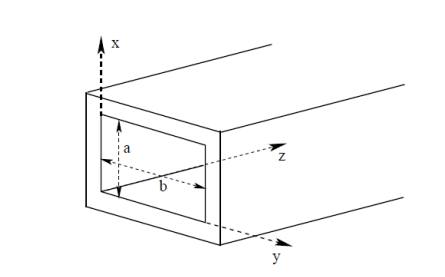
\includegraphics[width=0.4\textwidth]{schéma_guide_d'ondes.png}
  \label{fig:schéma_guide_'ondes}
\end{figure}
\begin{enumerate}
    \item Montrer que $f$ ne dépend que de y puis déterminer l'équation différentielle à laquelle est soumise $f(y)$.
    \item Résoudre cette équation et introduire un entier $n$ correspondant à différents modes propres. 
    \item Déterminer $\vec{B}$. $\vec{E}$ et $\vec{B}$ sont ils en phase ? 
    \item Exprimer $k_g$ en fonction de $\omega$, c, n et b. En déduire $\lambda_g$ en fonction de $\lambda_0$, b et n.
    \item Montrer qu’il existe une fréquence de coupure $f_c$ en dessous de laquelle il n’y a plus propagation.
    \item Exprimer la vitesse de phase $v_\phi$ de l’onde en fonction de c, n et du rapport $\frac{f}{f_c}$, $f$ étant la fréquence de l'onde.
    \item  Donner l’expression du vecteur de Poynting $\vec{\Pi}$ . Quelle est
    la valeur moyenne  $<\vec{\Pi}>$ dans le temps de ce vecteur ?
    En déduire la puissance moyenne transmise par une section droite du guide d’ondes.
    \item Calculer la valeur moyenne, dans le temps de la densité d’énergie volumique de l’énergie
    électromagnétique $<u>$
    \item A l’aide des résultats précédents, déduire la vitesse de propagation $v_e$ de l’énergie.
    Quelle relation simple peut-on constater entre $v_e $ et $v_\phi$ ? \\[2cm]
\end{enumerate}
\section{Oscillations d'une particule chargée}
Une charge accélérée rayonne un champ électromagnétique dans l'espace. On donne le vecteur de Poynting à une distance r de la charge: $\vec{\Pi} = \frac{\mu_0 q^2}{16\pi ^2 r^2 c} \|\vec{e_r} \wedge \frac{d\vec{v}}{dt}\|^2\vec{e_r}$, avec $v$ la vitesse de la particule. L'expression est évaluée en $u=t-\frac{r}{c}$
\begin{enumerate}
    \item En considérant le cas où la particule décrit une trajectoire rectiligne avec un mouvement harmonique, déterminer le vecteur de Poynting en fonction des coordonnées sphériques, puis sa moyenne temporelle. 
    \item Déterminer la puissance rayonnée dans tout l'espace. 
    \item Pourquoi le ciel est-il bleu ?
    \item Une particule chargée est suspendue à un ressort de raideur $k$ au bout duquel elle effectue des oscillations d'amplitude $x_0$ dont on donnera la pulsation. Calculer l'énergie mécanique moyenne de la particule. 
    \item Montrer que $x_0$ dépend nécessairement du temps, puis trouver sa loi de variation. 
\end{enumerate}
\end{document}



\section{Exercice 1}

\section{Exercice 2}

\section{Exercice 3}

\section{ Formulaire }

\end{document}